% hc2hp.tex

\documentclass[tikz]{standalone}
\usetikzlibrary{positioning, fit}

\begin{document}
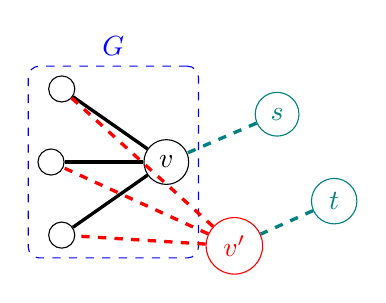
\begin{tikzpicture}[n/.style = {draw, circle, minimum size = 8pt}, 
  every edge/.style = {draw, very thick}, node distance = 0.6cm and 1.0cm]
  \node (v) [n] {$v$};

  \node (u1) [n, left = of v] {};
  \node (u2) [n, above left = of v] {};
  \node (u3) [n, below left = of v] {};

  \path (v) edge (u1)
  			edge (u2)
  			edge (u3);

  \node (g) [draw, dashed, blue, rectangle, rounded corners, fit = (v) (u1) (u2) (u3), label = {[blue] above : $G$}] {};

  \node (v') [n, red, below right = 0.6cm and 0.4cm of v] {$v'$};
  \path (v') edge[red, dashed] (u1)
			 edge[red, dashed] (u2)
			 edge[red, dashed] (u3);

  \node (s) [n, teal, above right = 0.2cm and 1.0cm of v] {$s$};
  \node (t) [n, teal, above right = 0.1cm and 0.8cm of v'] {$t$};
  \path (s) edge[teal, dashed] (v)
		(t) edge[teal, dashed] (v');
\end{tikzpicture}
\end{document}
